\documentclass[11pt,a4paper]{article}

\usepackage[margin=2.5cm]{geometry}
\usepackage{amsmath,amssymb}
\usepackage{booktabs}
\usepackage{graphicx}
\usepackage{subcaption}
\usepackage{multirow}
\usepackage{float}
\usepackage{hyperref}

\title{Supplementary Material\\[4pt]\large Variational Koopman Autoencoder Network with Mori--Zwanzig Closure for Stable and Interpretable Dynamics Learning}
\author{}
\date{\today}

\begin{document}

\maketitle

\section{Burgers Equation}

\begin{table}[H]
    \centering
    \caption{Forecast MAE at last time step for the Burgers case.}
    \label{tab:burgers-results}
    \begin{tabular}{lcccc}
        \toprule
        Method & VKAN & FNO & DeepOnet & Transformer \\
        \midrule
        Error   & 0.00061 & 0.00249 & 0.00357 & 0.00251 \\
        \bottomrule
    \end{tabular}
\end{table}

\begin{figure}[H]
    \centering
    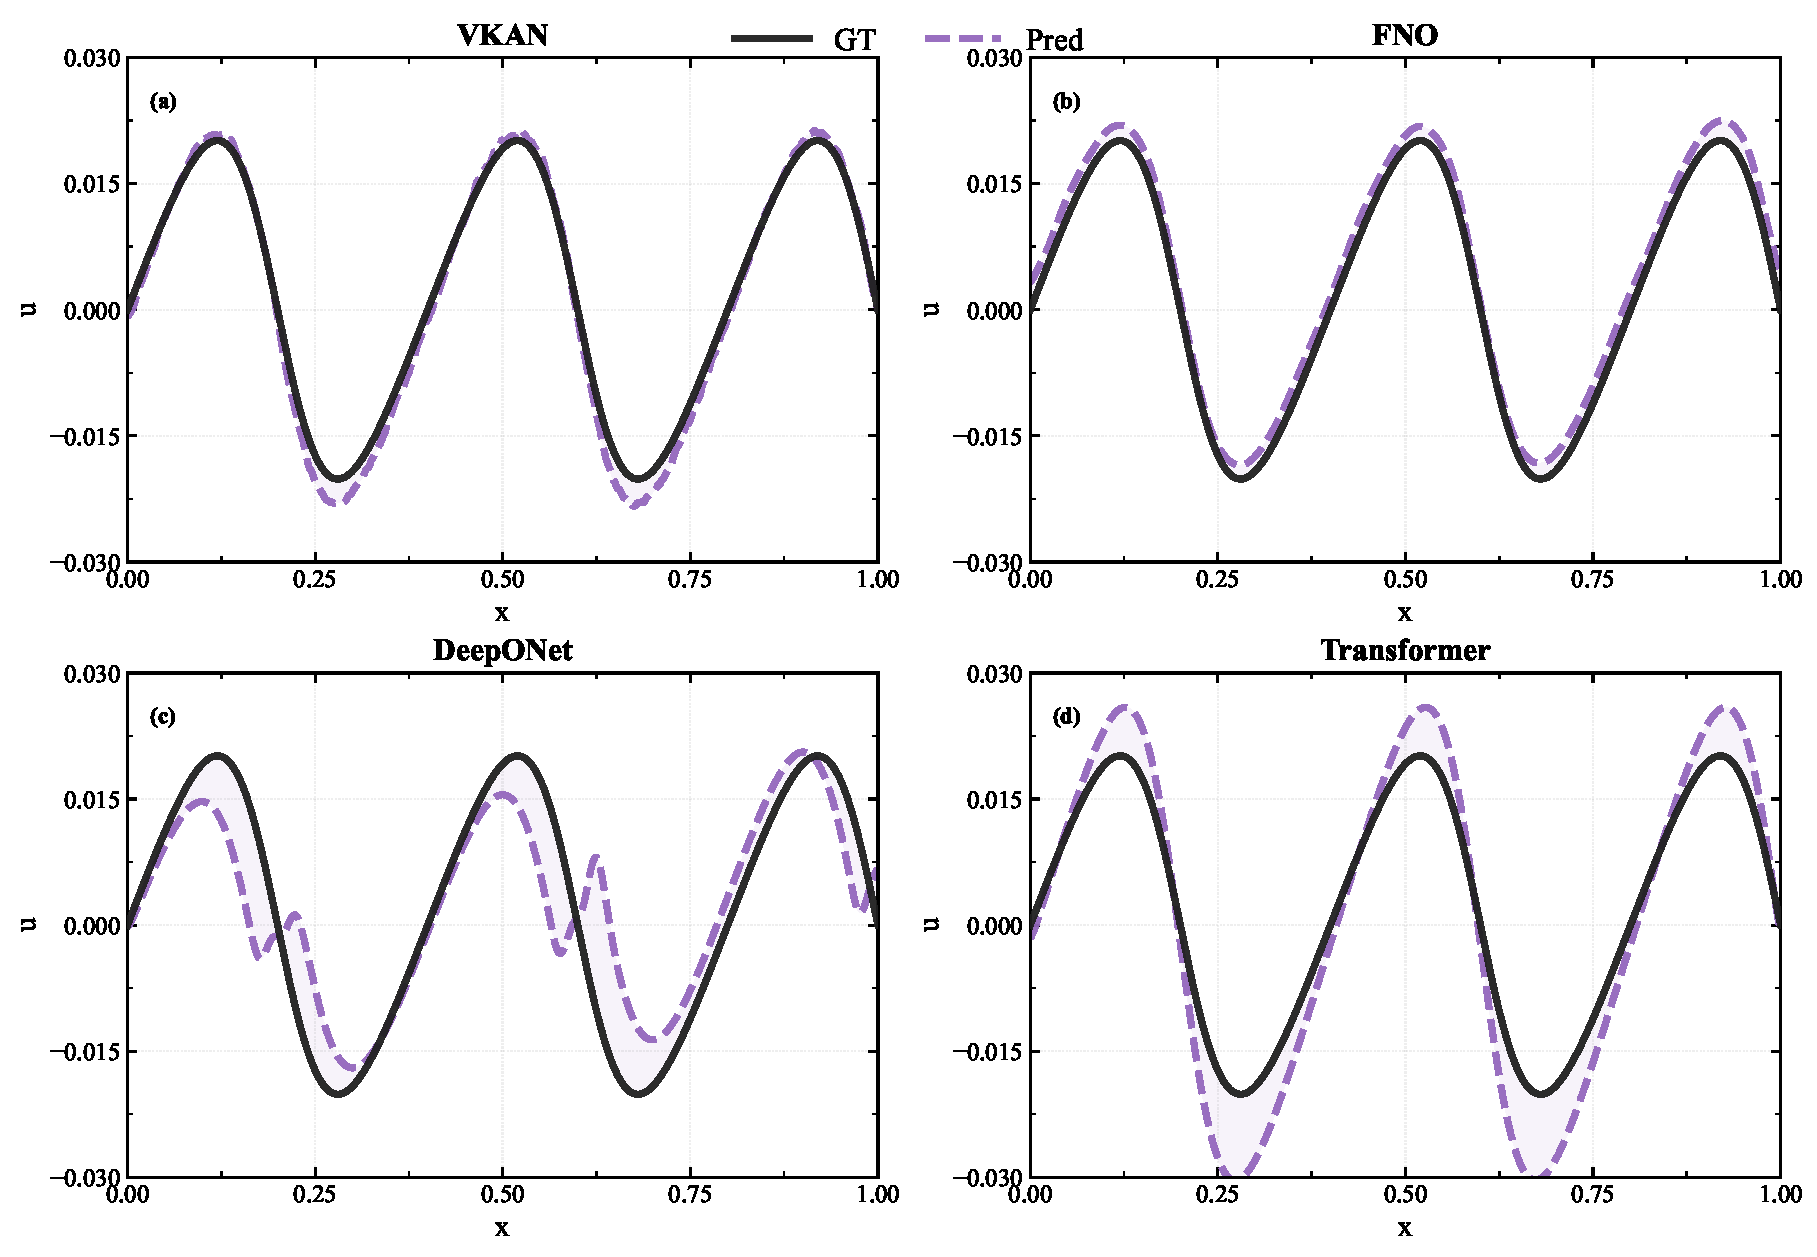
\includegraphics[width=0.95\textwidth]{burgers_case.pdf}
    \caption{Qualitative result for the Burgers case.}
    \label{fig:burgers-results}
\end{figure}


\section{Flow Past Cylinder}

\begin{table}[H]
    \centering
    \caption{Forecast MAE at last time step for the Cylinder flow.}
    \label{tab:cylinder-results}
    \begin{tabular}{lcccc}
        \toprule
        Method & VKAN & Deepkoopman & CKAE & KoVAE \\
        \midrule
        Error   & 0.0395 & 0.0686 & 0.0761 & 0.0736 \\
        \bottomrule
    \end{tabular}
\end{table}


\begin{figure}[H]
    \centering
    \includegraphics[width=0.7\textwidth]{cylinder_flow.pdf}
    \caption{Qualitative result for the cylinder flow.}
    \label{fig:cylinder-results}
\end{figure}

\section{Kuramoto--Sivashinsky Equation}

\begin{figure}[H]
    \centering
    \includegraphics[width=0.7\textwidth]{ks_train_forecast_triptych.pdf}
    \caption{Qualitative result for the Kuramoto--Sivashinsky equation.}
    \label{fig:ks-results}
\end{figure}

\end{document}
